\begin{figure*}[t]
\centering
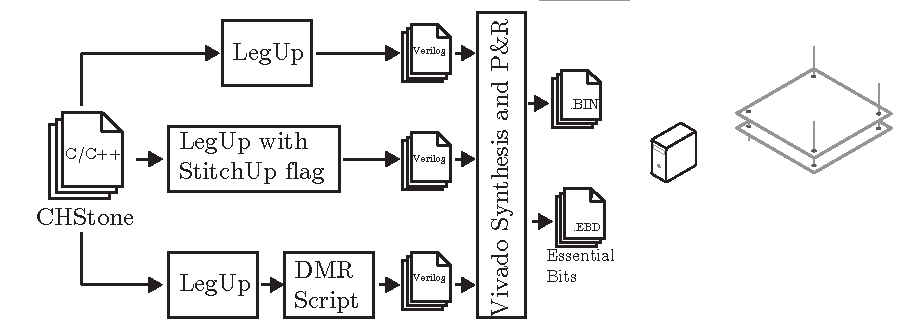
\includegraphics[width=6in]{./imgs/ExperimentFlow.pdf}
\caption{The experiment flow}
\label{fig:ExperimentFlow}
\end{figure*}

To test the error mitigation abilities of StitchUp generated circuits we have adopting the
gold standard of hardware fault injection, where configuration bits on the 
FPGA device are flipped from their original state.
Typical FPGA designs will require a large number of configuration bits often making
full exhaustive testing infeasible, usually resulting in the adoption of random
testing.
However in our case we have developed an experiment
platform allowing us to achieve full exhaustive fault injection in reasonable time
and where possible we have used this to test StitchUp on the popular CHStone 
HLS benchmarks.

We make use of many low cost Xilinx FPGA SoC devices known as
Zedboards all injecting on the same circuit in parallel.
Each Zedboard runs a full Linux OS on its hardened ARM processor and is arranged into
a cluster managed by a single desktop\footnote{called The SoC Drawer}.

To flip individual configuration bits a Xilinx Soft Error Mitigation (SEM) IP Core
connected to the FPGA internal configuration port (ICAP) was used and
targeting Xilinx devices was possible due to the latest release of LegUp
(v4.0) which has the ability to generate generic Verilog circuits.
For each experiment the SEM core and the test circuit were instantiated and connected to the
ARM processing system via AXI interconnects.
Software running under Linux on each of the ARM cores marshaled each test by, sending the
address and injection command to the SEM core, starting the circuit under test, and
collecting the results.

Figure \ref{fig:ExperimentFlow} shows an overview of the experiment setup.
The top flow generates a standard LegUp circuit with no protection;
as the middle uses StitchUp to generate a control-flow structure protected circuit;
and the bottom generates a full DMR protected circuit duplicating the original LegUp
circuit and generating comparison logic on the control FSM state register;

Each different version is then passed through the Xilinx FPGA circuit tool flow to produce
two files, an essential bits file (.EBD), and a configuration binary (.BIN).
The essential bits file is a list of configuration memory bits that have any
influence on our generated circuit and is used to reduce the number of injections
required to fully test our design.\footnote{essential bits do not contain BRAM data,
since these are considered transient data not essential}
For each experiment the EBD files are divided up into smaller chunks and each chunk is
processed in parallel on a different Zedboard device.

\subsection{Performing the error injection}
Software running on the ARM of each Zedboard marshals each test by, injecting a fault,
running the circuit, and storing the result.
The injected fault is then repaired by re-injecting an error into the
same configuration memory location (i.e. flipping the bit back to it's original state).
Some fault may cause the circuit to never terminate so if no response is seen within three orders
of magnitude of it's expected time a timeout halts its execution and keeps a record of it.

The results are then analysed and each outcome is classified into three separate categories:

\begin{enumerate}
\setlength{\itemsep}{1pt}
\setlength{\parskip}{0pt}
\setlength{\parsep}{0pt}
\item Execution Time Error \textbf{ETE} - This is where the execution of the circuit either took
an incorrect number of cycles to complete or timed out. Errors of these type are
control flow related since any deviation from the correct execution path will cause
an incorrect number of cycles.
\item Data-Flow Only Errors \textbf{DOE} - These are errors where the circuit has returned an incorrect
data result but has executed in the correct number of cycles, such as error caused
by faults in a non-control structure functional unit.
\item Caught Errors \textbf{CE} - These are errors in the state register that were detected by the protection method, which is
either DMR or StitchUp.
\end{enumerate}
